% UNet Decoder Implementation Correction
\documentclass{article}
\usepackage{graphicx}
\usepackage{amsmath}
\usepackage{booktabs}
\usepackage{listings}
\usepackage{xcolor}
\usepackage{hyperref}
\usepackage{tikz}
\usetikzlibrary{shapes.geometric, arrows, positioning, fit}

\title{UNet Decoder Implementation: Skip Connection Correction}
\author{Distillation Trajectories Project}
\date{\today}

\begin{document}

\maketitle

\section{Introduction}

This document details an important correction to the U-Net decoder implementation in our StudentUNet architecture. The correction addresses a channel dimension mismatch that occurs specifically when using the "full" architecture type with certain size factors (notably 0.7). Understanding this issue is crucial for correctly implementing U-Net architectures with skip connections in the context of diffusion models.

\section{The Problem: Decoder Channel Dimension Mismatch}

In U-Net architectures, skip connections between encoder and decoder paths are a fundamental component that helps maintain spatial detail in the output. During implementation, it's critical to correctly calculate the input channel dimensions for decoder blocks after concatenating features from the skip connections.

\subsection{The Bug}

In our original implementation, the input channel calculation for decoder blocks incorrectly assumed that when concatenating features in the decoder path, we were combining:

\begin{enumerate}
  \item Upsampled features from the previous decoder layer (with dims[i] channels)
  \item Skip connection from the previous encoder level (with dims[i-1] channels)
\end{enumerate}

This was implemented as:

\begin{lstlisting}[language=Python, frame=single]
# Decoder blocks
self.decoder_blocks = nn.ModuleList()
for i in range(len(self.dims)-1, 0, -1):
    in_channels = self.dims[i] + self.dims[i-1]  # Skip connection + previous layer
    out_channels = self.dims[i-1]
    self.decoder_blocks.append(Block(in_channels, out_channels, self.time_emb_dim))
\end{lstlisting}

However, this was inconsistent with what was actually happening in the forward pass:

\begin{lstlisting}[language=Python, frame=single]
# Decoder pathway with skip connections
for i, block in enumerate(self.decoder_blocks):
    x_current = self.upsample(x_current)
    skip_idx = len(skip_connections) - i - 1
    skip_connection = skip_connections[skip_idx]
    
    # Ensure dimensions match before concatenation
    if x_current.shape[2:] != skip_connection.shape[2:]:
        x_current = F.interpolate(x_current, size=skip_connection.shape[2:], 
                                  mode='bilinear', align_corners=True)
    
    x_current = torch.cat([x_current, skip_connection], dim=1)
    x_current = block(x_current, time_emb)
\end{lstlisting}

\subsection{The Error}

The error manifested as a dimension mismatch when applying the student model with a size factor of 0.7, resulting in the error:

\begin{lstlisting}[basicstyle=\small\ttfamily, breaklines=true, frame=single]
RuntimeError: Given groups=1, weight of size [96, 280, 1, 1], expected input[128, 368, 16, 16] to have 280 channels, but got 368 channels instead
\end{lstlisting}

With size factor 0.7, the model dimensions were [96, 184, 184, 184]. The discrepancy between expected and actual channel dimensions was large enough to cause a runtime error.

\section{The Correct Implementation}

\subsection{Understanding Skip Connections in U-Net}

In the correct U-Net implementation, at each decoder level, we concatenate:

\begin{enumerate}
  \item Upsampled features from the bottleneck or previous decoder layer (with dims[i] channels)
  \item Skip connection from the same level encoder (with dims[i] channels)
\end{enumerate}

This results in an input with 2 * dims[i] channels.

\subsection{The Fix}

The corrected implementation calculates the decoder block input channels as:

\begin{lstlisting}[language=Python, frame=single]
# Decoder blocks
self.decoder_blocks = nn.ModuleList()
for i in range(len(self.dims)-1, 0, -1):
    in_channels = self.dims[i] + self.dims[i]  # Skip connection + current level features
    out_channels = self.dims[i-1]
    self.decoder_blocks.append(Block(in_channels, out_channels, self.time_emb_dim))
\end{lstlisting}

This correctly accounts for the actual concatenation happening in the forward pass.

\section{Implications and Lessons}

\subsection{U-Net Architecture Principles}

This correction highlights several important principles when implementing U-Net architectures:

\begin{enumerate}
  \item Skip connections link encoder and decoder at the same level
  \item Input channels for decoder blocks must account for both upsampled features and skip connections
  \item Channel dimension calculations must be consistent between model initialization and forward pass
\end{enumerate}

\subsection{Diagram of Correct Skip Connection Pattern}

\begin{center}
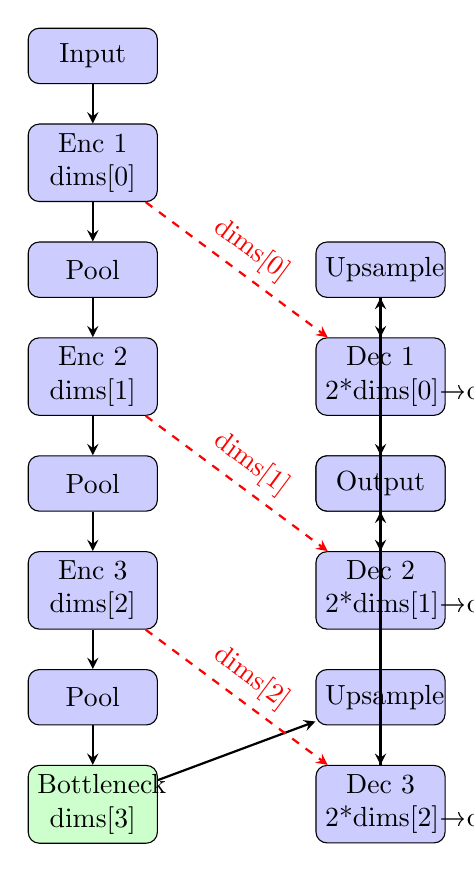
\begin{tikzpicture}[
    block/.style={rectangle, draw, fill=blue!20, text width=4em, text centered, rounded corners, minimum height=2em},
    arrow/.style={thick,->,>=stealth},
    skipconn/.style={dashed, thick,->,>=stealth, red}
]

% Encoder path
\node[block] (in) {Input};
\node[block, below=0.5cm of in] (enc1) {Enc 1 \\ dims[0]};
\node[block, below=0.5cm of enc1] (pool1) {Pool};
\node[block, below=0.5cm of pool1] (enc2) {Enc 2 \\ dims[1]};
\node[block, below=0.5cm of enc2] (pool2) {Pool};
\node[block, below=0.5cm of pool2] (enc3) {Enc 3 \\ dims[2]};
\node[block, below=0.5cm of enc3] (pool3) {Pool};

% Bottleneck
\node[block, below=0.5cm of pool3, fill=green!20] (bottle) {Bottleneck \\ dims[3]};

% Decoder path
\node[block, below right=0.5cm and 2cm of enc3] (up3) {Upsample};
\node[block, below=0.5cm of up3] (dec3) {Dec 3 \\ 2*dims[2]→dims[1]};
\node[block, below right=0.5cm and 2cm of enc2] (up2) {Upsample};
\node[block, below=0.5cm of up2] (dec2) {Dec 2 \\ 2*dims[1]→dims[0]};
\node[block, below right=0.5cm and 2cm of enc1] (up1) {Upsample};
\node[block, below=0.5cm of up1] (dec1) {Dec 1 \\ 2*dims[0]→out};
\node[block, below=0.5cm of dec1] (out) {Output};

% Connections
\draw[arrow] (in) -- (enc1);
\draw[arrow] (enc1) -- (pool1);
\draw[arrow] (pool1) -- (enc2);
\draw[arrow] (enc2) -- (pool2);
\draw[arrow] (pool2) -- (enc3);
\draw[arrow] (enc3) -- (pool3);
\draw[arrow] (pool3) -- (bottle);

\draw[arrow] (bottle) -- (up3);
\draw[arrow] (up3) -- (dec3);
\draw[arrow] (dec3) -- (up2);
\draw[arrow] (up2) -- (dec2);
\draw[arrow] (dec2) -- (up1);
\draw[arrow] (up1) -- (dec1);
\draw[arrow] (dec1) -- (out);

% Skip connections
\draw[skipconn] (enc3) -- node[above, sloped] {dims[2]} (dec3);
\draw[skipconn] (enc2) -- node[above, sloped] {dims[1]} (dec2);
\draw[skipconn] (enc1) -- node[above, sloped] {dims[0]} (dec1);

\end{tikzpicture}
\end{center}

\section{Why Size Factor 0.7 Revealed the Bug}

With size factor 0.7, the model dimensions were calculated as [96, 184, 184, 184]. This specific combination of dimensions highlighted the bug because:

\begin{enumerate}
  \item At each decoder level, the upsampled feature maps had 184 channels
  \item The skip connections also had 184 channels from the corresponding encoder level
  \item When concatenated, this resulted in 368 channels
  \item However, the decoder block was incorrectly initialized expecting 184 + 96 = 280 channels
  \item This mismatch of 368 vs 280 channels triggered the runtime error
\end{enumerate}

With other size factors, the dimensions might have been more "forgiving" or the scaling might have resulted in dimensions that worked coincidentally.

\section{Conclusion}

This document has detailed an important architectural correction in our implementation of the U-Net decoder blocks for diffusion models. The fix ensures proper handling of skip connections and channel dimensions, which is crucial for proper model operation. This correction is particularly important when working with scaled-down student models in knowledge distillation scenarios, where architectural details must be precisely maintained despite changing model dimensions.

Understanding the correct flow of data and corresponding channel dimensions in U-Net architectures is essential for implementing effective diffusion models, especially when applying scaling factors to modify model size.

\end{document} 